\documentclass{article}

\usepackage[utf8]{inputenc}
\usepackage{titlesec}
\PassOptionsToPackage{hyphens}{url}\usepackage{hyperref}
\usepackage{listings}
\usepackage{graphicx}
\usepackage{float}
\usepackage{xcolor}
\usepackage{csquotes}
\usepackage{lettrine}


\title{ First Report of Semantic Web about \\ \Huge \textbf{Food}}
\author{Aspir Ahmet \\ Tobias Dick \\ Daniel Egger \\Stefan Kaufmann}
\date{05.11.2018}


\begin{document}
\thispagestyle{empty}
\clearpage
\maketitle
\thispagestyle{empty}
\thispagestyle{empty}
\newpage
\clearpage
\tableofcontents 
\thispagestyle{empty}
\newpage
\pagebreak
\pagenumbering{arabic}
	
\section{Introduction}
This Knowledge-Graph based application will serve as a online Recipe-Look-Up service. Either by entering certain ingredients, cook time, an old fashioned search query or all of the previously mentioned, the request will yield according results. A web-overlay ensures the interaction with regular users. \\ \\
The motivation behind this project has a few points that need to be addressed. The first would be the fact that all the ingredients at home do not get wasted, so before buying new ones it would make sense to look up recipes that would require all the ingredients already in possession. 
The other point is there to help out busy people or lazy students that do not want to spend too much time on a dish. \\ \\
The project will be based on various data-sources that are gathered all across the world wide web. These sources are stored locally in order to utilize search queries on them without having the delay  when consulting external sources. To be precise the gathered data will be mapped onto a vocabulary that is initially selected from $<$schema.org$>$. One aim is to expand the selected vocabulary either by defining new relations by ourselves or using parts of already existing ontologies and merging it together with the already existing one. Once the data is ready it is going to be stored in a TripleStore of choice so valid SPARQL query can give us certain triples. One candidate is Apache Jena Fuseki which is a HTTP based TripleStore that can be accessed by a Java-Client.
Once the back-end is ready the goal is to develop a front-end for end-users.
	
\section{Domain Overview}
\subsection{Description}
The topic of this project is simply FOOD. We are focusing on recipes for everyday users which will easy obtain their much desired result. Since there are a lot of properties a recipe can hold we tried to keep it very simple by cutting away things like nutrition. Our ultimate goal is to focus on ingredients and cook-time.
\subsection{Data Sources}
On the search for data-sources we stumbled upon on a lot very different options. After we got our first data-source we were on the lookout for more sources and found this blog post:
\href{https://medium.com/groceristar/companies-with-recipe-apis-e9f29a64389c?fbclid=IwAR1cqotmvKyCeA13FEYZwN4p20LB1531emcffBYFMrwe01jOpdQ19CnHCUg}{click here for the Blog}.\\ \\
The author basically describes different APIs and recipe-based data-sources and gives a short review for each of them. For now are main suppliers are EDAMAM API (1.7+ million recipes), RECIPE-PUPPY API (10.000+ recipes) and a source we found laying on a Amazon-Web-Server (518 recipes). \\ \\
The data we got was in JSON-format but Edamam also had an own ontology. Since we decided to use $<$schema.org$>$ as our base we ultimately decided to map every JSON source to JSON-LD. 

\section{Initial Vocabulary Selection and Domain Specification}
\subsection{Initial vocabulary}
Our first idea was to use schema.org because of its popularity. We were able to find a schema.org class that fits our intentions. The main class is $<$\url{https://schema.org/Recipe}$>$ as seen in Figure \ref{fig:initvoc}.

\begin{figure}[H]
  \centering
  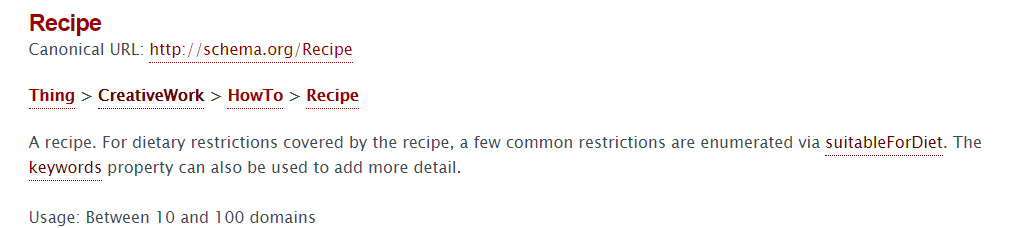
\includegraphics[width=12cm]{pictures/init_voc.png}
  \caption{The Recipe class of schema.org}
  \label{fig:initvoc}
\end{figure}
\noindent
The properties of this class already covered most of our wanted vocabulary (Figure \ref{fig:initvoc2}). There were also some properties we used that were not directly related to this class but seemed nonetheless important to ourselves.

\begin{figure}[H]
  \centering
  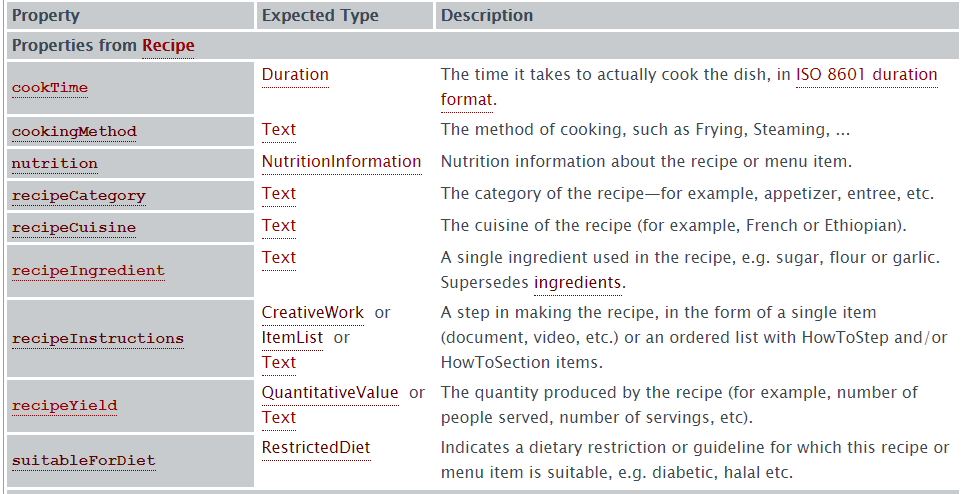
\includegraphics[width=10cm]{pictures/init_voc2.png}
  \caption{Properties of the Recipe class}
  \label{fig:initvoc2}
\end{figure}
\noindent

\subsection{Mapping of metadata of the source to the selected vocabularies/ontologies}
The Edamam API provides a JSON result in the structure as seen in Figure \ref{fig:map}.

\begin{figure}[H]
  \centering
  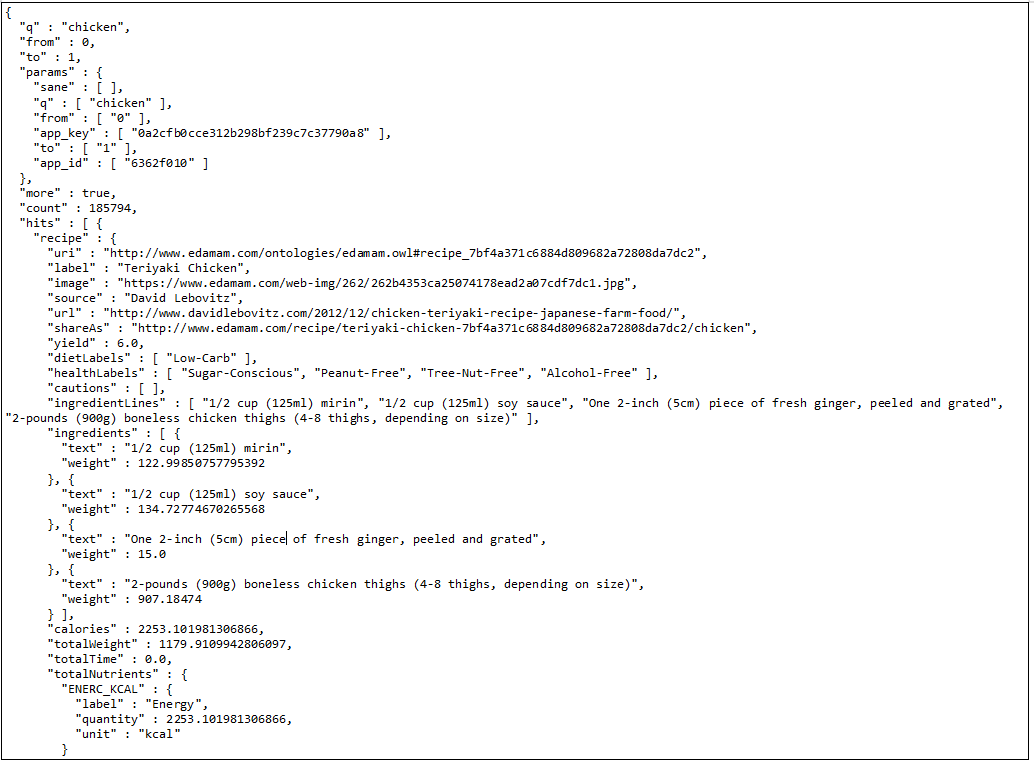
\includegraphics[width=12cm]{pictures/mapping.png}
  \caption{A JSON result from the Edamam API}
  \label{fig:map}
\end{figure}
\noindent
A summary of the mapping:

\begin{figure}[H]
  \centering
  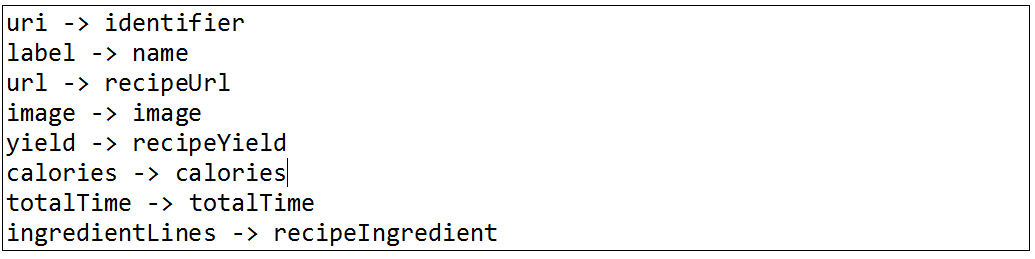
\includegraphics[width=12cm]{pictures/mapping_sum.png}
  \label{fig:mapsum}
\end{figure}
\noindent

\subsection{Implementation of mapper tool}
Using a java program both the crawler and mapper were implemented. In the snippets below the function call can be seen that sends an HTTP request to the API, reads the JSON result, parses it and maps it to our own vocabulary. Finally a simple string is generated which represents the JSON-LD file (LINE 151+).

\begin{figure}[H]
  \centering
  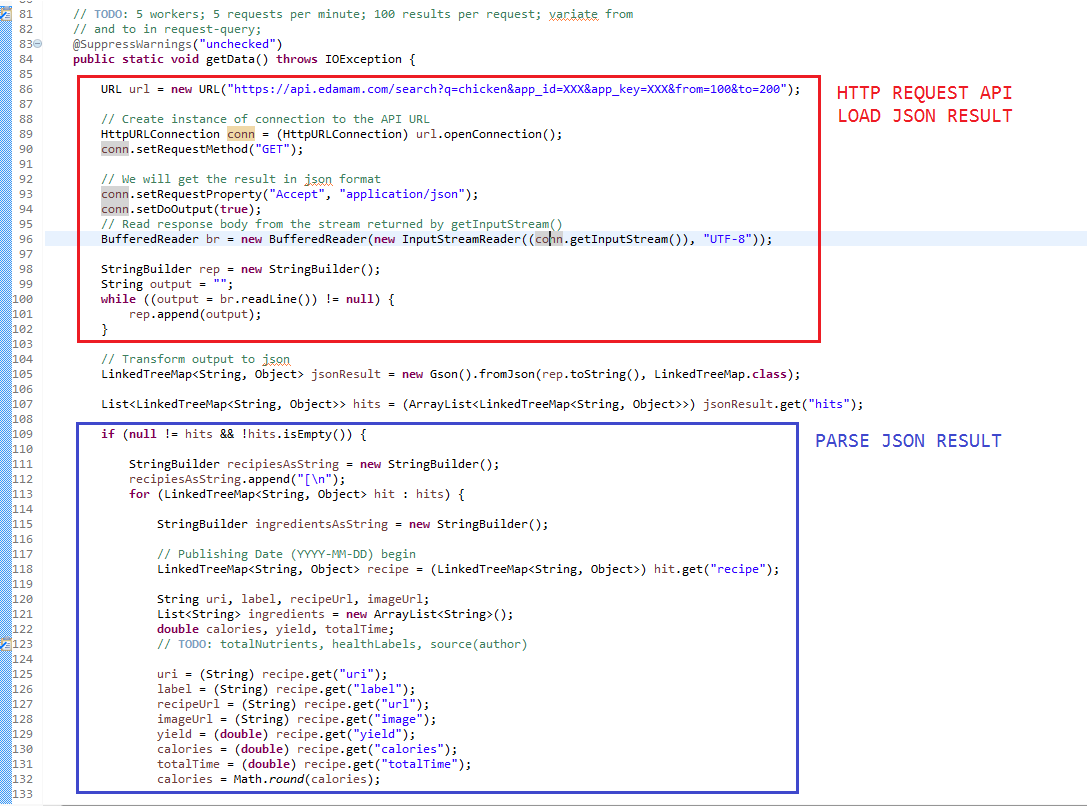
\includegraphics[width=12cm]{pictures/mapping_tool.png}
  \label{fig:maptool}
\end{figure}

\begin{figure}[H]
  \centering
  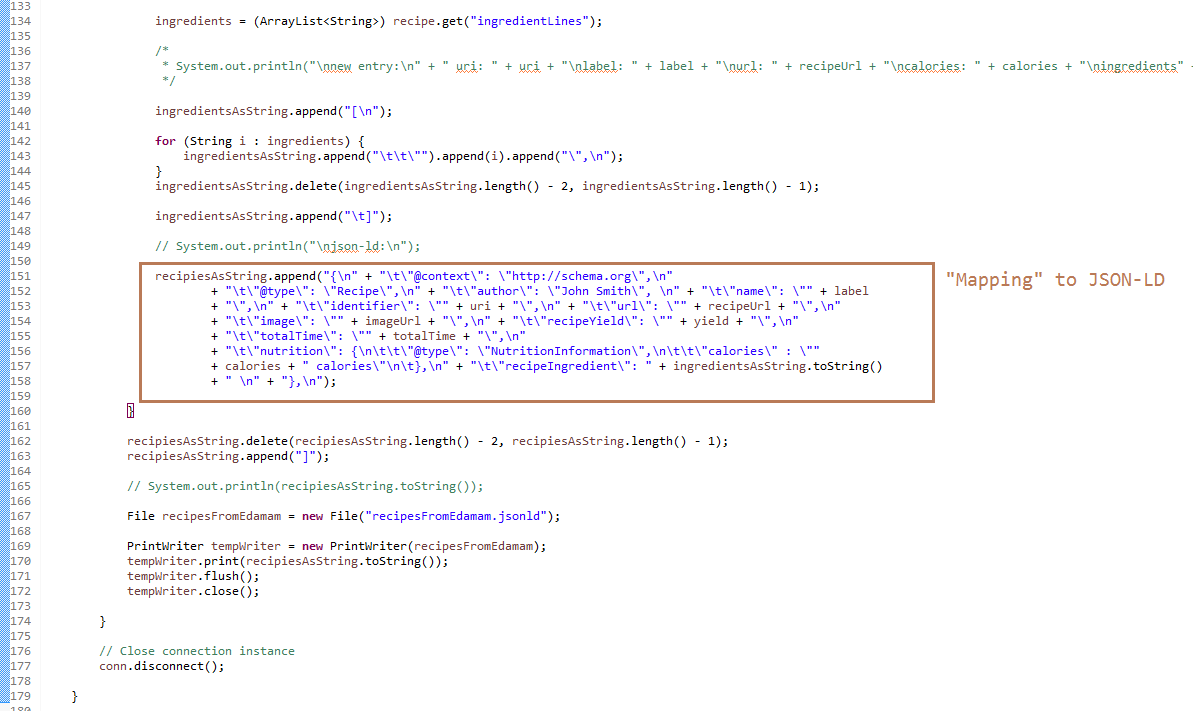
\includegraphics[width=12cm]{pictures/mapping_tool2.png}
  \label{fig:maptool2}
\end{figure}
\noindent

\subsection{Implementation of crawler tool}
The crawler is basically the previous function call wrapped in to a Callable class in Java so the data gathering can happen simultaneously. One thing is important to keep in mind: the Edamam API restricts the calls per minute and results per request. \\ \\
With 5 available calls per minute and only 100 results per request we have to implement a tiny waiting routine and a flexible selection of results. This is done by tweaking the parameters $<$FROM$>$ and $<$TO$>$ in the API request call. \\ \\
In the following example 100 and 200: \url{https://api.edamam.com/search?q=chicken&app_id=XXX&app_key=XXX&from=100&to=200}

\begin{figure}[H]
  \centering
  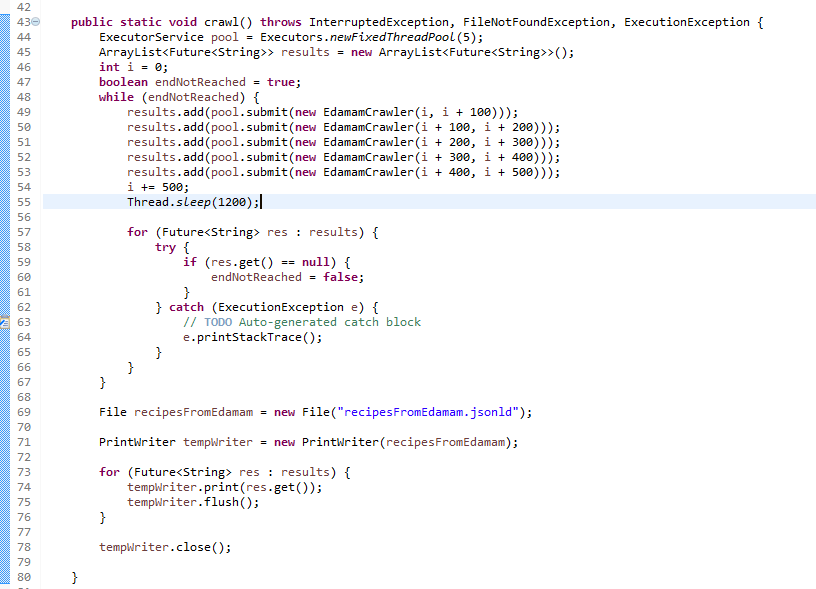
\includegraphics[width=13cm]{pictures/crawler_tool.png}
  \caption{The Crawler Implementation}
  \label{fig:crawl}
\end{figure}
\newpage

\subsection{Ontology extension}
Since the selected properties are not classes themselves we will try to make a class out of recipeIngredient for example. Currently the information for this property is stored as a String but it would make sense to introduce properties like \enquote{amount} and \enquote{name} and maybe some more attributes for this new class (Figure \ref{fig:vocext}).

\begin{figure}[H]
  \centering
  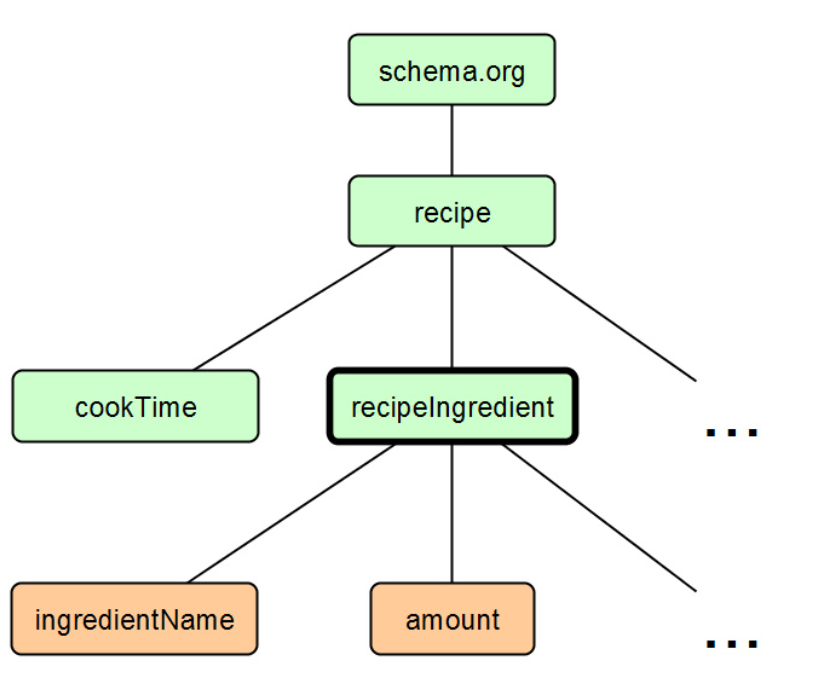
\includegraphics[width=7cm]{pictures/voc_ext.png}
  \caption{The Described extension-point of the Recipe class}
  \label{fig:vocext}
\end{figure}
\newpage

\section{Exploratory queries on the loaded dataset}
\subsection{Small overview of the selected triple store}
The selected TripleStore is Apache Jena  Fuseki (\url{https://jena.apache.org/documentation/fuseki2/}). \\ \\
We are using the HTTP TripleStore from Jena, because its easy to handle from a Java client. For now Fuseki is launched from a separate path and runs on localhost on port 3030 and provides a GUI via web (Figure \ref{fig:fuseki}). 

\begin{figure}[H]
  \centering
  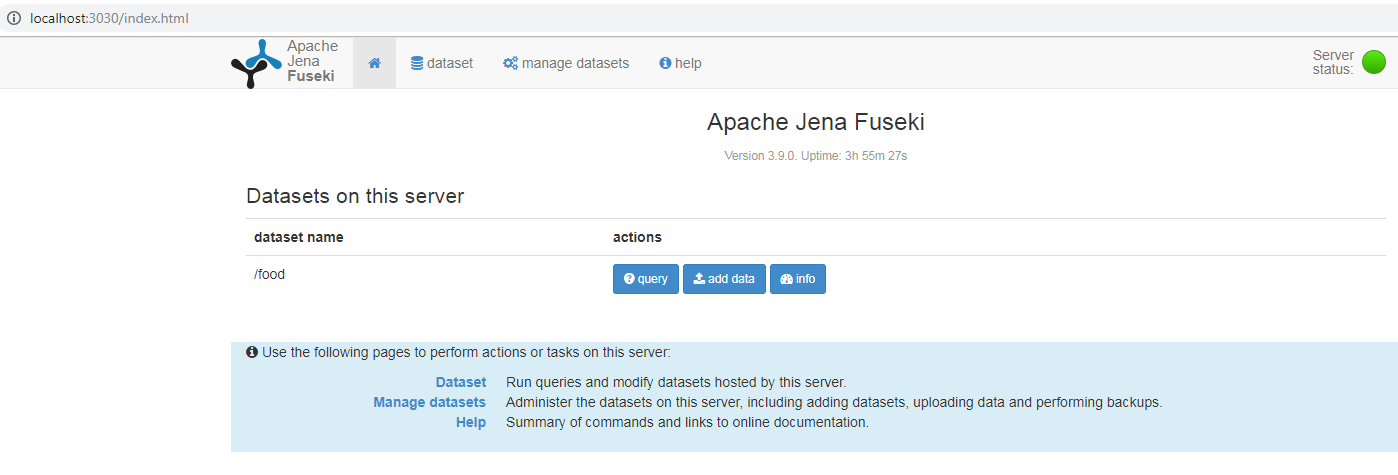
\includegraphics[width=12cm]{pictures/fuseki.png}
  \caption{The Apache Jena Fuseki GUI}
  \label{fig:fuseki}
\end{figure}
\noindent
Pretty much everything can be done with the Java client if the permissions are granted. Fuseki usually has endpoints that can be accessed for certain operations (Figure \ref{fig:fusekiserv}). \\

\begin{figure}[H]
  \centering
  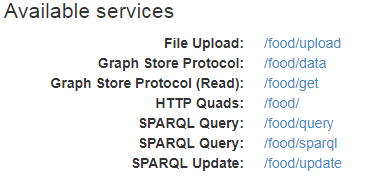
\includegraphics[width=12cm]{pictures/fuseki_services.png}
  \caption{The Apache Jena Fuseki services}
  \label{fig:fusekiserv}
\end{figure}
\noindent
Once graphs are loaded they can be stored on hard disk or the main memory depending on the purpose. For our purposes we kept our graphs on the hard disk. The data-set that's on the fuseki is easily accessed by local methods can be seen in Figure \ref{fig:fusekild} and Figure \ref{fig:fusekisparql} below.

\begin{figure}[H]
  \centering
  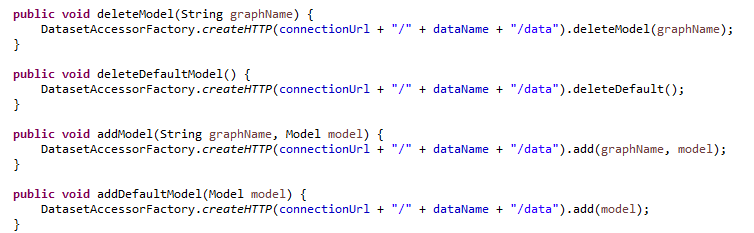
\includegraphics[width=12cm]{pictures/fuseki_loadDelete.png}
  \caption{Load and delete operations on desired graphs}
  \label{fig:fusekild}
\end{figure}
\noindent
The SPARQL query is deployed in a method which requires the query itself as a string.

\begin{figure}[H]
  \centering
  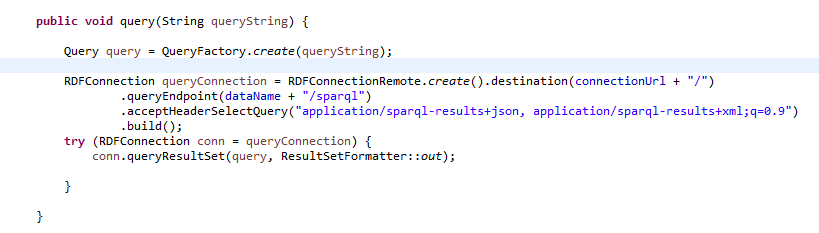
\includegraphics[width=12cm]{pictures/fuseki_conn.png}
  \caption{Deploying a SPARQL query}
  \label{fig:fusekisparql}
\end{figure}
\newpage

\subsection{Example query}
We want to have a small section were we explain the thought process behind our queries. The general setup are named graphs for data sources and ontologies. Union of all named graphs is currently the default graph (not really needed since we are very flexible with our queries). \\ \\
Example query with detailed explanation: Get all classes from data-set (data-set is a single movie entry).

\begin{figure}[H]
  \centering
  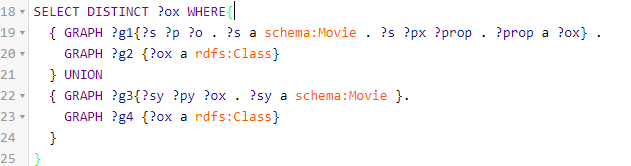
\includegraphics[width=12cm]{pictures/example_query.png}
  \label{fig:exqu}
\end{figure}
\noindent
The query above is the solution for this and is explained in each step. \\ \\
The GRAPH keyword goes trough the named graphs and binds one of them to the subset within the parentheses. That means if the ontologies need to be accessed this has to be done outside with a separate GRAPH call.\\ \\
The key idea behind this query is to first get each subjects that have the rdf:type schema:Movie.

\begin{figure}[H]
  \centering
  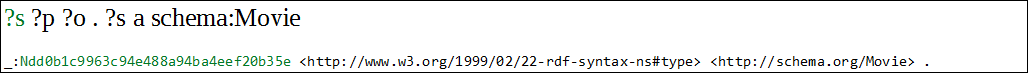
\includegraphics[width=12cm]{pictures/example_query2.png}
  \label{fig:exqu2}
\end{figure}
\noindent
This way we can be sure that our GRAPH is bound to the named graph which contains the data. From there we have to find each objects where a reference from the main subject can be back traced. We assume that from the main subject there are certain predicates that address properties.

\begin{figure}[H]
  \centering
  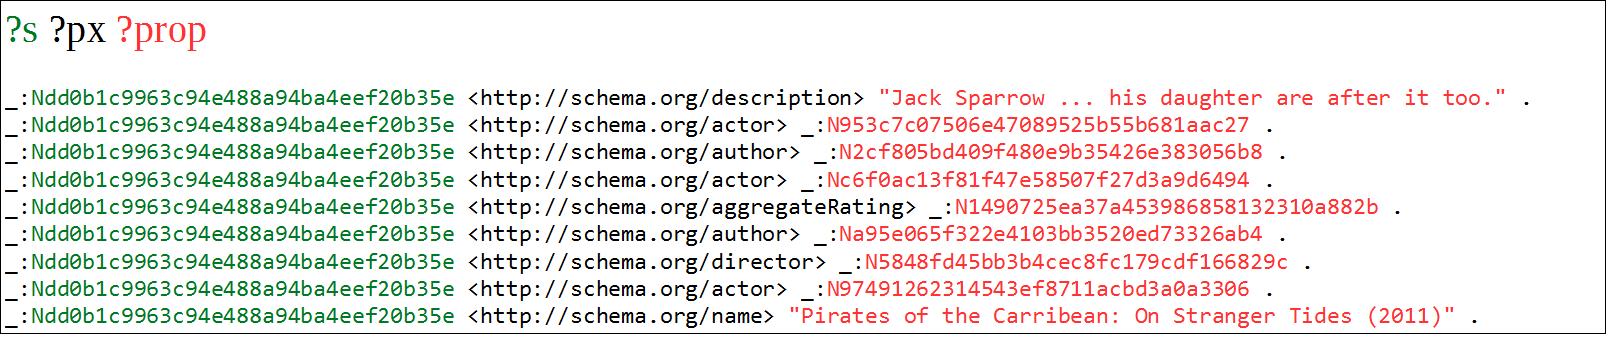
\includegraphics[width=12cm]{pictures/example_query3.png}
  \label{fig:exqu3}
\end{figure}
\noindent
Next up we want to determine the type of the objects \textcolor{red}{?prop} that are mentioned in the main movie subject and get all \textcolor{orange}{?ox}.

\begin{figure}[H]
  \centering
  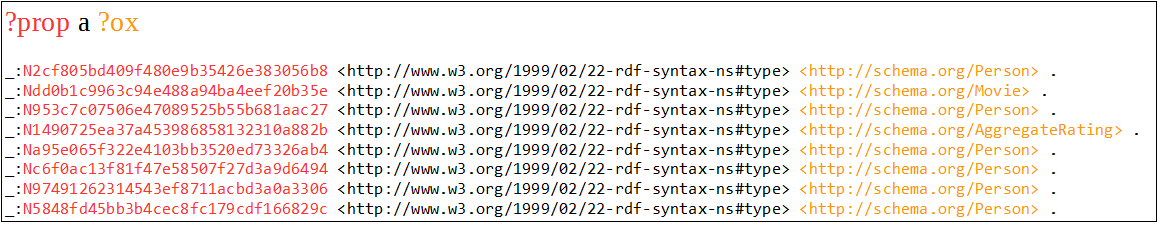
\includegraphics[width=12cm]{pictures/example_query4.png}
  \label{fig:exqu4}
\end{figure}
\noindent
Once we get the needed results from the dataset its up to the second named graph which is the ontology to find out if the results are rdfs:Class types. For the example we just show it for schema:Person.

\begin{figure}[H]
  \centering
  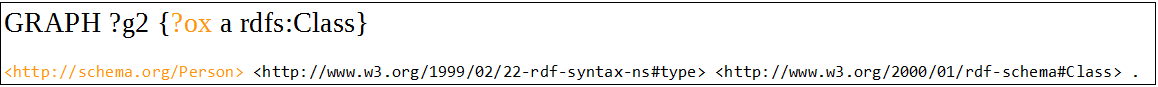
\includegraphics[width=12cm]{pictures/example_query5.png}
  \label{fig:exqu5}
\end{figure}
\noindent
The second part of the query is to ensure we get the movie class itself as well. This is done by utilizing the keyword UNION. Union means there are two sets to select the results from. If only one column is desired keep the variable name same, otherwise write the variable names of each subset in the SELECT.

\begin{figure}[H]
  \centering
  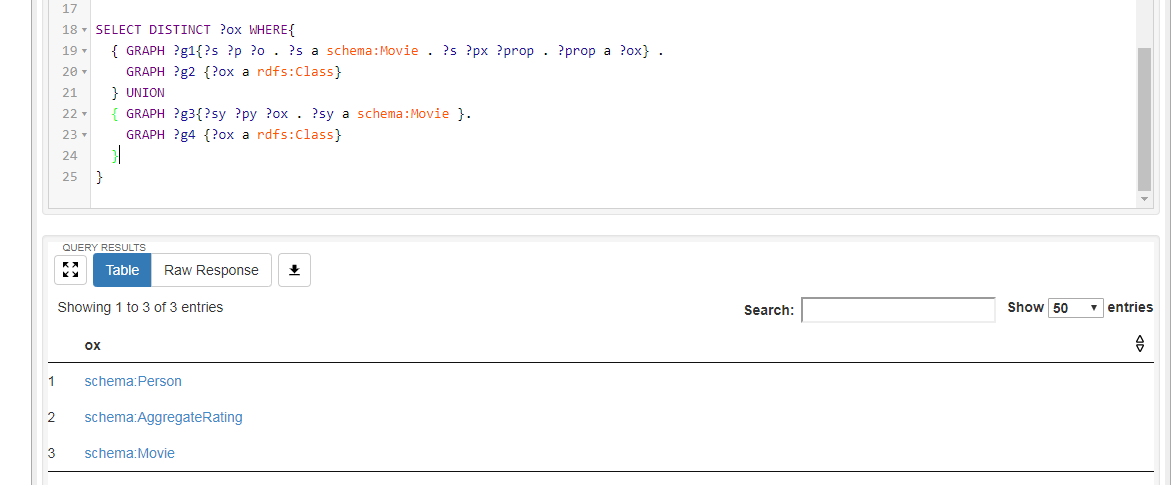
\includegraphics[width=12cm]{pictures/example_query_result.png}
  \label{fig:exqures}
\end{figure}
\newpage


\subsection{Results of exploratory queries}
In this section we want to show the constructed SPARQL-queries including their results.
\subsubsection{Total number of triples}

\begin{figure}[H]
  \centering
  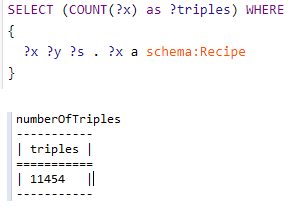
\includegraphics[width=10cm]{pictures/res1_triples.png}
  \label{fig:qures1}
\end{figure}

\subsubsection{Total number of instantiations}

\begin{figure}[H]
  \centering
  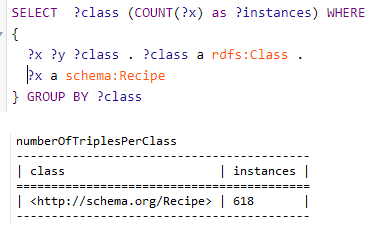
\includegraphics[width=12cm]{pictures/res2_instantiations.png}
  \label{fig:qures2}
\end{figure}

\subsubsection{Total number of distinct classes}

\begin{figure}[H]
  \centering
  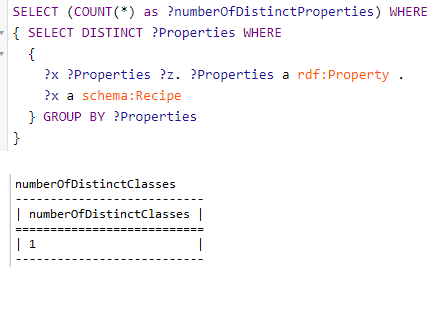
\includegraphics[width=12cm]{pictures/res3_dist_classes.png}
  \label{fig:qures3}
\end{figure}

\subsubsection{Total number of distinct properties}

\begin{figure}[H]
  \centering
  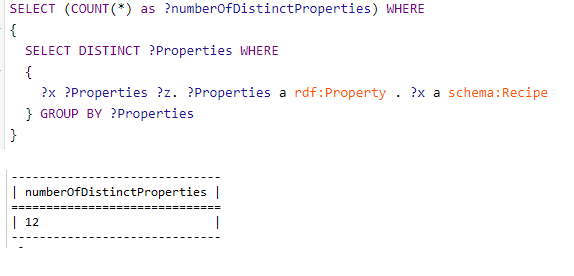
\includegraphics[width=12cm]{pictures/res4_dist_prop.png}
  \label{fig:qures4}
\end{figure}

\subsubsection{List of all classes used in dataset per data source}

\begin{figure}[H]
  \centering
  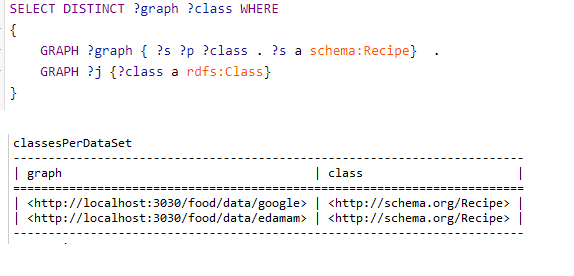
\includegraphics[width=12cm]{pictures/res5_classes_per_datasource.png}
  \label{fig:qures5}
\end{figure}

\subsubsection{List of all properties used in dataset per data source}

\begin{figure}[H]
  \centering
  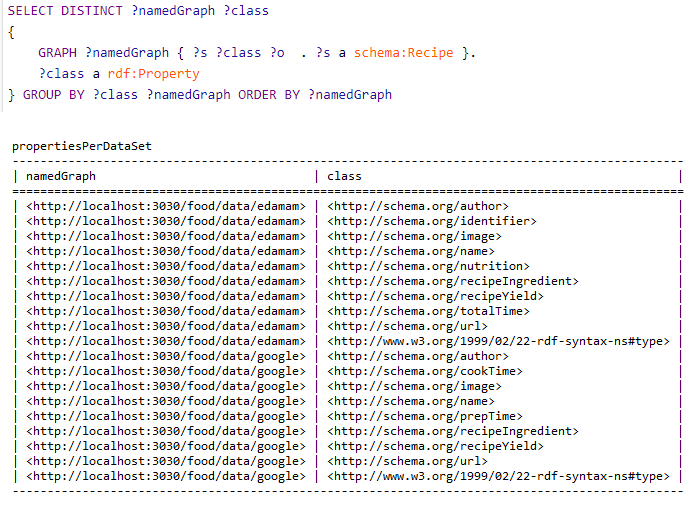
\includegraphics[width=12cm]{pictures/res6_prop_per_datasource.png}
  \label{fig:qures6}
\end{figure}

\subsubsection{Total number of instances per class per data source}

\begin{figure}[H]
  \centering
  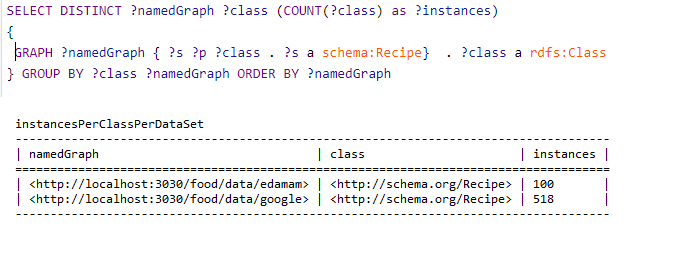
\includegraphics[width=12cm]{pictures/res7_inst_per_class_per_datasource.png}
  \label{fig:qures7}
\end{figure}

\subsubsection{Total number of distinct subjects per property per data source}

\begin{figure}[H]
  \centering
  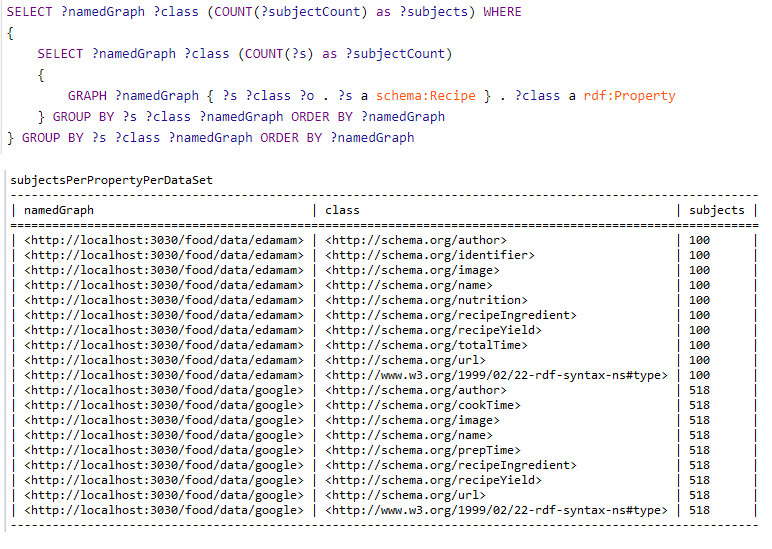
\includegraphics[width=13cm]{pictures/res8_sub_per_class_per_datasource.png}
  \label{fig:qures8}
\end{figure}

\subsubsection{Total number of distinct objects per property per data source}

\begin{figure}[H]
  \centering
  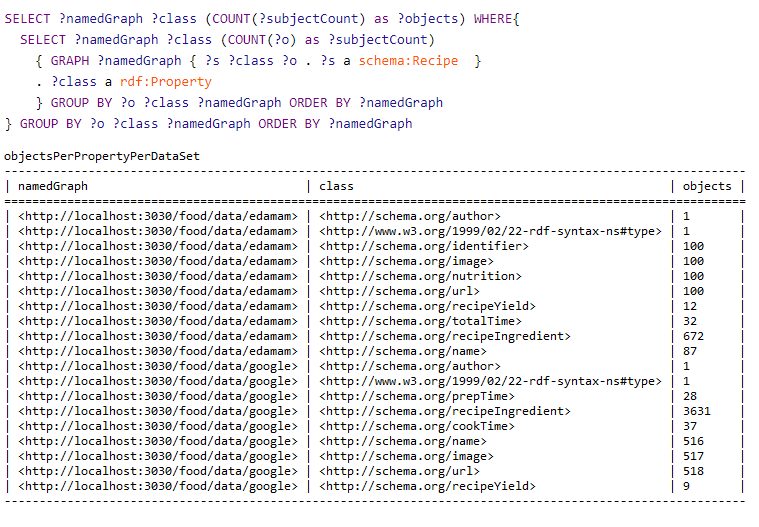
\includegraphics[width=12cm]{pictures/res9_obj_per_class_per_datasource.png}
  \label{fig:qures9}
\end{figure}

\subsubsection{Distinct properties used on top 5 classes}

\begin{figure}[H]
  \centering
  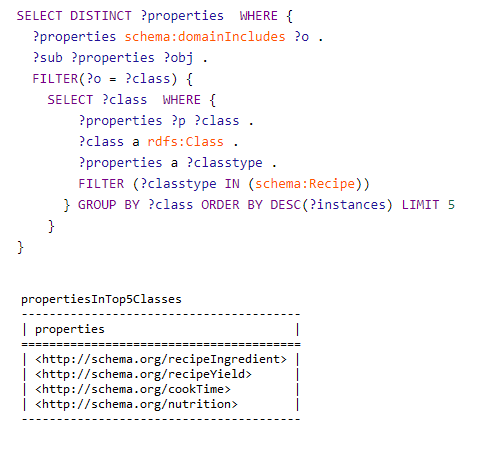
\includegraphics[width=8cm]{pictures/res10_dist_prop_of_top5_classes.png}
  \label{fig:qures10}
\end{figure}

\subsubsection{Distinct wikidata types that may be aligned with}

\begin{figure}[H]
  \centering
  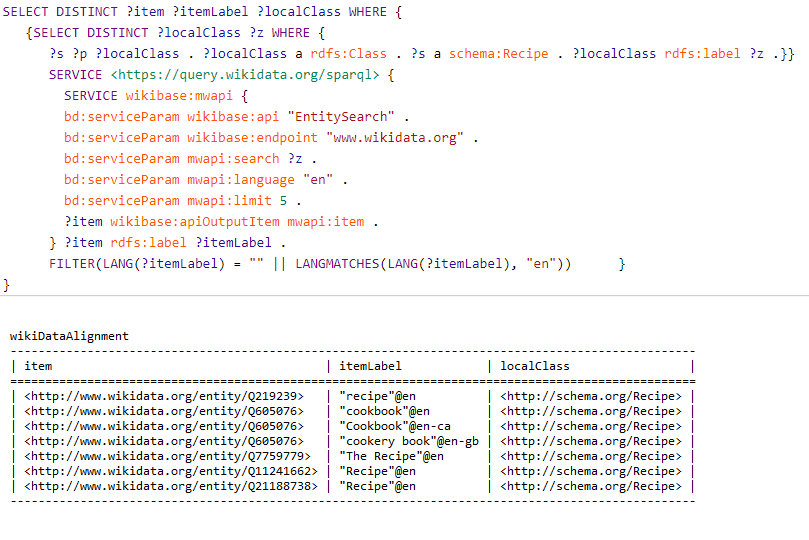
\includegraphics[width=12cm]{pictures/res11_align_wikidata.png}
  \label{fig:qures11}
\end{figure}
	
\section{Conclusion and Next Steps}
The application is up and running and is available to give back results for certain criteria when asked. The aim was to have a functioning TripleStore with data that represents an ontology so semantics can be applied to raw data. Querying the data via SPARQL and a Java client also works well and will most definitely not hinder us on further progress. A milestone was to get the requested queries to run which we accomplished. What we need to focus on is to extend the current vocabulary we are using and also think of a possible framework for the frontend.

	

\end{document}	